\documentclass{article}

% Essential packages
\usepackage{graphicx}   % For image handling
\usepackage{subcaption} % For multi images
\usepackage{caption}    % For proper captions
\usepackage{listings}   % For code listings
\usepackage{fontspec}   % For custom fonts
\usepackage{xcolor}     % For color support
\usepackage{tcolorbox}  % For code block boxes
\usepackage{etoolbox}   % For patching and command manipulation
\usepackage{titlesec}   % For section formatting
\usepackage{parskip}    % For customisable paragraph formating
\usepackage{comment}    % For being able to comment out sections
\usepackage{geometry}   % For managing page size and margins
\usepackage{hyperref}   % For embedding links, like URL's
\usepackage{amsmath}    % For math and equation formatting

\tcbuselibrary{listings, skins, breakable}  %Librarary to make code blocks multipage


%   ############################## Customisation ##############################

% Document metadata
\title{\fontsize{24}{36}\selectfont PB1010 - Fysikk 1\\ %Edit title here \\ means new line
Oblig 1} % Line 2 of title, its not subtitle, that is possible to, google it
\author{Sølve Kjelseth} % Input your name
\date{\today} % Auto updates the date, untill you export it, replace with hardcoded date if you need

% Adjust the body text font size to 12pt without affecting section headings
\renewcommand{\normalsize}{\fontsize{12}{16}\selectfont}

% Adjust the paragraph spacing, either as indentation or/and line spaceing
\setlength{\parindent}{0pt}  % Remove indentation
\setlength{\parskip}{6pt}    % Add vertical space between paragraphs

% Customisation of fonts and colors
\setmainfont{Times New Roman}
\setmonofont{JetBrains Mono}
\definecolor{background}{RGB}{225, 219, 202}
\definecolor{darkAccent}{RGB}{140, 98, 64}
\definecolor{commentGreen}{RGB}{26, 159, 32}
\definecolor{keywordPurple}{RGB}{229, 24, 192}
\definecolor{keywordBlue}{RGB}{5, 142, 217}
\definecolor{portOrange}{RGB}{234, 72, 31}
\definecolor{darkGray}{RGB}{60, 60, 60}

% Link color customization
\hypersetup{
    colorlinks=true,
    linkcolor=darkGray, % Internal links such as table of contents or figure referencing
    urlcolor=keywordBlue % URL colors
    }
\urlstyle{same} % Makes url in the same style as the rest of the document

% Customisation of margins and paper size
\geometry{
 a4paper,
 left = 30mm,
 right = 30mm,
 top = 30mm,
 bottom = 30mm
 }

% Sections formatting and numbering
% Sets the font to monospace for section, subsection and subsubsection
% and sets the format to be numbers with . between and at the end
\renewcommand{\thesection}{\texttt{\arabic{section}.}}
\renewcommand{\thesubsection}{\texttt{\arabic{section}.\arabic{subsection}.}}
\renewcommand{\thesubsubsection}{\texttt{\arabic{section}.\arabic{subsection}.\arabic{subsubsection}.}}

\setcounter{section}{-1}  % Start section numbering from 0, delete this to start from 1

% Makes section monospace font and start each subsection from 0 and figure number
\let\oldsection\section
\renewcommand{\section}[1]{%
  \oldsection{\texttt{#1}} % Make section title monospace
  \setcounter{subsection}{-1} % Makes subsection start from 0, delete this line to start from 1
  \setcounter{figure}{-1} % Makes figure numbers start from 0, delete this line to start from 1
}

% Makes subsection monospace font and start each subsubsection from 0
\let\oldsubsection\subsection
\renewcommand{\subsection}[1]{%
  \oldsubsection{\texttt{#1}}% Make subsection title monospace
  \setcounter{subsubsection}{-1}% Makes subsubsection start from 0, delete this line to start from 1
}

% Makes subsubsection monospace font
\let\oldsubsubsection\subsubsection
\renewcommand{\subsubsection}[1]{%
  \oldsubsubsection{\texttt{#1}}% Make subsubsection title monospace
}

% Makes every new section start on a new page, except for the first section, section 0
\pretocmd{\section}{%
  \ifnum\value{section}=-1 \else\clearpage\fi % Replace -1 with 0 if sections start at nr. 1
}{}{}

% Makes Table of contents a subsection
\makeatletter
\renewcommand{\tableofcontents}{%
    \subsection{Table of Contents} % Numbered subsection named Table of contents
    \@starttoc{toc}%
}
\makeatother

% Makes List of figures a subsection
\makeatletter
\renewcommand{\listoffigures}{%
    \subsection{List of Figures} % Numbered subsection named List of figures
    \@starttoc{lof}%
}
\makeatother

% Makes every figure be formated as section number.figure number
\renewcommand{\thefigure}{\arabic{section}.\arabic{figure}}

% Add keywords to be highlited in blue below. Note that all reserved
% keywords from VHDL is already in purple and should not be added here
% too as duplicates will cause issues. Therfore compile this document
% after pasting in code and only add non-highlited words to this list.
% Also, there is not a list for orange keywords, used for ports here.
\lstdefinelanguage{VHDL+}{
    language     = VHDL,
    morestring = [b]',
    morekeywords = [2]{
        IEEE,
        std_logic_1164, std_logic, std_logic_vector},
    morekeywords = [3]{
        SW, LEDR, KEY,
        HEX0, HEX1, HEX2, HEX3, HEX4, HEX5, HEX6},
    sensitive = false
}

\lstdefinelanguage{Python+}{
    language     = Python,
    morekeywords = [2]{
        None, ValueError},
    morekeywords = [3]{
        self},
    sensitive = true
}


%   ############################## Advanced customisation ##############################

% Customisation of list style inside code block
\lstdefinestyle{VHDL}{
    language = VHDL+, % Uses the extra higlights from above
    % The folloowing lines defines color for highlighting, other changes like
    % italic, bold or different fonts can also be added to this
    commentstyle = \color{commentGreen}, 
    keywordstyle = \color{keywordPurple},
    keywordstyle = [2]\color{keywordBlue},
    keywordstyle = [3]\color{portOrange},
    stringstyle = \color{darkAccent},
    basicstyle = \ttfamily\small, % Default font inside code block
    numberstyle = \ttfamily\color{darkAccent}, % Style of line numbering
    numbers = left, % Line numbering on left side
    breakatwhitespace = false, % Don't start new line with only whitspaces
    breaklines = true, % If line is to long it will wrap to next line (line number does not increase)
    keepspaces = true, % Indents works logical
    showspaces = false, % Space is blank character, set to true to show dots instad
    showstringspaces = false, % Same as above but inside strings
    showtabs = false, % Tab is also blank character, set to true to show dashes
    tabsize = 4, % Tabsize is set to 4, this works well with code from notepad++
    % Dont mess with the ones below unless you want to mess with the box as well
    % These took some time to line up such that it looks natural
    numbersep = 10pt, % Adjust distance between numbers and code
    xleftmargin = -8pt,% Negative margin to pull code text closer to the left border
}

\lstdefinestyle{Python}{
    language = Python+, % Uses the extra higlights from above
    % The folloowing lines defines color for highlighting, other changes like
    % italic, bold or different fonts can also be added to this
    commentstyle = \color{commentGreen}, 
    keywordstyle = \color{keywordPurple},
    keywordstyle = [2]\color{keywordBlue},
    keywordstyle = [3]\color{portOrange},
    stringstyle = \color{darkAccent},
    basicstyle = \ttfamily\footnotesize, % Default font inside code block
    numberstyle = \ttfamily\color{darkAccent}, % Style of line numbering
    numbers = left, % Line numbering on left side
    breakatwhitespace = false, % Don't start new line with only whitspaces
    breaklines = true, % If line is to long it will wrap to next line (line number does not increase)
    keepspaces = true, % Indents works logical
    showspaces = false, % Space is blank character, set to true to show dots instad
    showstringspaces = false, % Same as above but inside strings
    showtabs = false, % Tab is also blank character, set to true to show dashes
    tabsize = 4, % Tabsize is set to 4, this works well with code from notepad++
    % Dont mess with the ones below unless you want to mess with the box as well
    % These took some time to line up such that it looks natural
    numbersep = 10pt, % Adjust distance between numbers and code
    xleftmargin = -8pt,% Negative margin to pull code text closer to the left border
}

% This is for code where VHDL is not an argument
\lstdefinestyle{Example Code}{
    basicstyle = \ttfamily\small, % Default font inside code block
    numberstyle = \ttfamily\color{darkAccent}, % Style of line numbering
    numbers = left, % Line numbering on left side
    breakatwhitespace = false, % Don't start new line with only whitspaces
    breaklines = true, % If line is to long it will wrap to next line (line number does not increase)
    keepspaces = true, % Indents works logical
    showspaces = false, % Space is blank character, set to true to show dots instad
    showstringspaces = false, % Same as above but inside strings
    showtabs = false, % Tab is also blank character, set to true to show dashes
    tabsize = 4, % Tabsize is set to 4, this works well with code from notepad++
    % Dont mess with the ones below unless you want to mess with the box as well
    % These took some time to line up such that it looks natural
    numbersep = 10pt, % Adjust distance between numbers and code
    xleftmargin = -8pt,% Negative margin to pull code text closer to the left border
}

\lstset{style = Example Code} %Sets the default style to Example Code

% Customisation of code block itself
\newtcolorbox[auto counter, number within=section]{codeBlock}[2][]{
    colback=background, % Background color for the code block
    colframe=darkAccent, % Border color for the code block
    listing only, %Makes it contain the listing
    arc=10pt, % Rounded corners size
    sharp corners=northeast, % Make top-right corner sharp for the main box
    enhanced jigsaw, % Essential dont mess with it
    breakable, % Allows content to be multipage
    top=-4pt, % Made to line up text dont mess with it
    bottom=-4pt, % Same as above
    before skip=0pt, after skip=10pt, % Adjust spacing before and after the box
    boxrule=1pt, % Border thickness of the main box
    overlay unbroken and first={\node[ % Create label box in the top-right corner
        anchor=north east,      %Position of box, same as sharp corner in this case
        fill=background,        %Background color same as main box
        draw=darkAccent,        %Outline color, same as main box
        line width=1pt,         %Outline thickness, same as main box
        text=keywordPurple,     %Text color
        font=\ttfamily,         %Text font and size
        inner sep=6pt,          %Spacing inside
        minimum width=16pt,     %Minimum box with, it autoresizes depending on text
        minimum height=12pt,    %Minimum box height, it autoresizes depending on text
        text centered,          %Centres the text with the spacing
        sharp corners]          %Makes corners sharp
        at ([xshift=0pt, yshift=0pt]frame.north east) % Position, aligned with corner on main box
        {#2}; % Types your argument in the top corner as a label
    }
}

% This is the custom command used for inserting code blocks
\newcommand{\writecode}[3][Example Code]{%
    \begin{codeBlock}{#1}% arg 1 (default Example Code) will be writtin in top right corner box
        \lstinputlisting[style=#1]{Code/#2}% arg 1 style is used and arg 2 is filename
    \end{codeBlock}%
    \begin{figure}[h] % Empty figure for captioning and referencing
        \centering
        \renewcommand\figurename{Code}
        %\captionsetup{type=figure, name=Code}
        \caption{#3} % arg 3 is used for caption
        \label{Code:#2} % Uniqe label for referencing is using file name
    \end{figure}
}

% This is the custom command used for making the introduction section
\newcommand{\introduction}[1][]{%
    \addtocontents{toc}{\protect\setcounter{tocdepth}{0}} % Temporarily hide from TOC
    \section{Introduction} % Numbered section named Introduction
    \ifx\relax#1\relax % Check if argument is empty
    \else
        #1 % Insert the optional text if provided
    \fi
    \tableofcontents % Generate TOC
    \clearpage
    \listoffigures % List of figures
    \addtocontents{toc}{\protect\setcounter{tocdepth}{2}} % Restore TOC depth
}



%   ############################## Document begins here ##############################

\begin{document}

\maketitle % Makes title front page based on the title, author and date metadata, change at the top


%           ########## Section ##########
% This makes the first section, introduction, that are excluded from the table of contents and
% has an optional text argument, then it creates table of contents and list of figures
\introduction[
This is for Oblig 1 in Physics where the mechanics of a free falling ball is dissected.\\
Note: The \LaTeX\ and python code is open source, \href{https://github.com/Kjelseth/Physics/tree/4eafb2ed19a347886ba41ad8a429e05fd7a3dd91/Fysikk1/Oblig1}{github link}.
]


%   ############################## Section ##############################
\section{Task 1}
I do not understand why the assignment wants to have ground level at \(h = 0m\) and positive direction downwards at the same time(as stated in part a), that means the sphere has a starting position at \(h = -50m\). The math works either way and even if it seems counterintuitive I choose to adhere to the requirements of the task and assumes this direction going forward unless otherwise stated.

\subsection{Part a}
To solve part a I choose to use the ISEE method.

\subsubsection{Identify}
I find some important variables, such as ground level, \(h_{ground} = 0m\) and distance between the ground and the sphere \(x_{sphere-ground} = 50m\). I also see that positive direction is downwards, that means \(h > 0\) will be meters under ground. That makes starting position \(h_0 = -50m\). Air resistance is omitted, this way only gravity affects acceleration. This is constant acceleration, downwards, thereby positive \(a = g = 9.825ms^{-2}\) (This is the official number for \(g\) in Oslo). Therefore the equations for motion in constant acceleration can be used. I also note that the start time of the free fall is at \(t_0 = 0s\) and it has no initial velocity \(v_0 = 0ms^{-1}\). Lastly I see that everything in this part is single dimension motion.

\subsubsection{Set up}
For the first question, find \(h(t)\), we know the goal variable is position, we "know" the time variable as all possible values will be put in, and finally the last known is acceleration. this means the velocity less equation can be used.

\begin{equation}
    x = x_0 + v_0t + \frac{1}{2}at^2
    \label{eq:noVel}
\end{equation}

For the next question, find \(v(t)\), we know the goal variable is velocity, and here time is also "known" as it is the function input and since we know acceleration as well the position less equation can be used.
\begin{equation}
    v = v_0 + at
    \label{eq:noPos}
\end{equation}

For the final question, find \(t_{ground}\), we can rearrange Equation~\ref{eq:noVel} to find the time when we calculate further. A sketch of the situation is provided on the next page.

\clearpage
\begin{figure}[h]
    \centering
    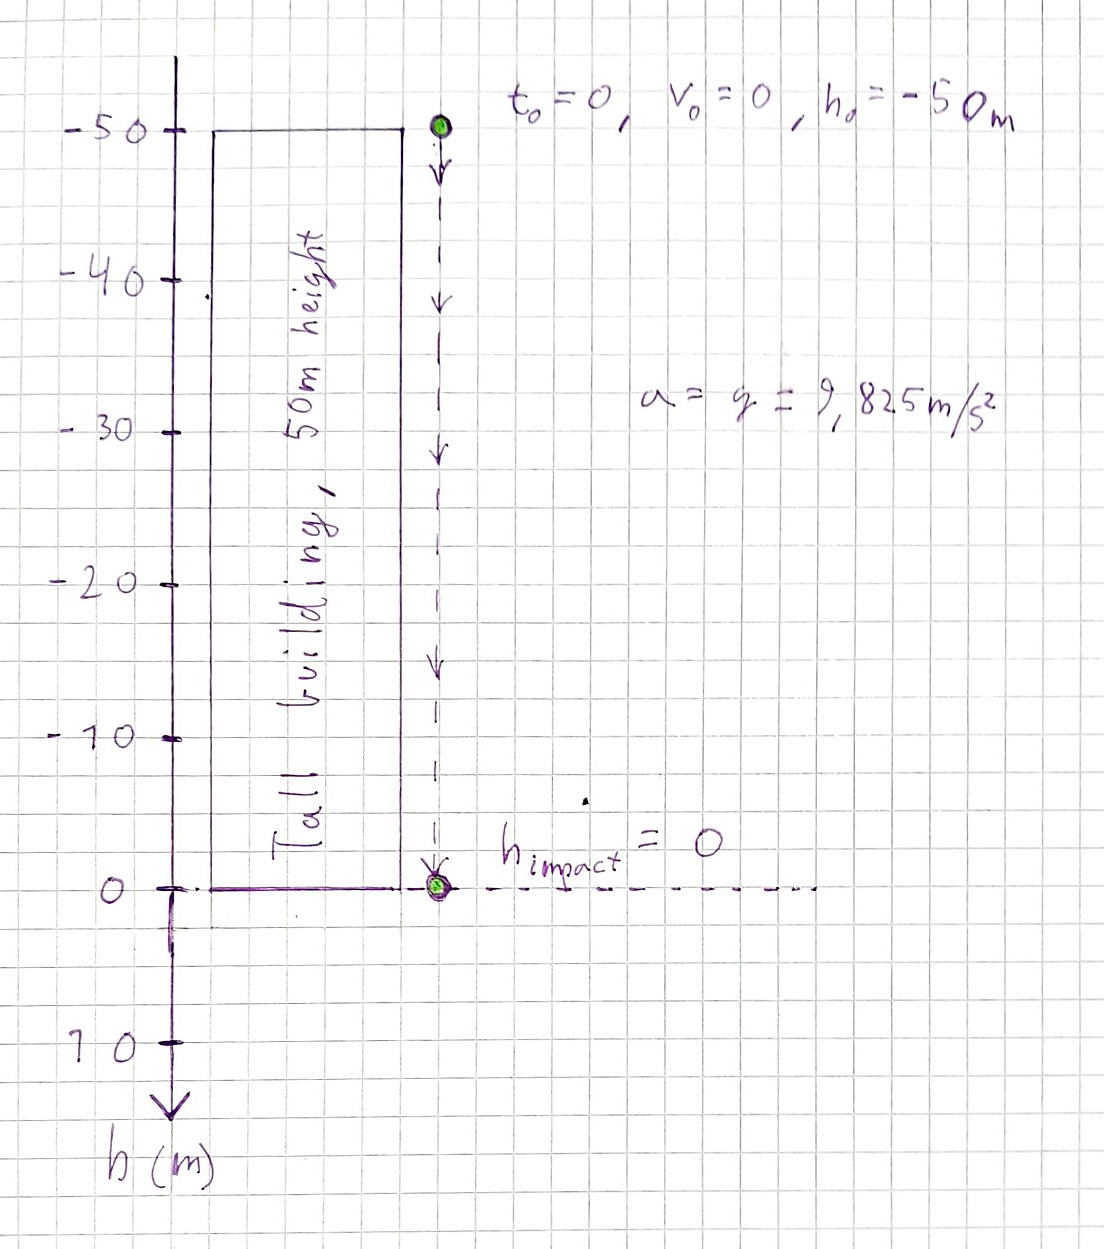
\includegraphics[width=0.6\textwidth]{Figures/Sketch1.jpg}
    \caption{Sketch of sphere falling from building}
    \label{fig:sketch_1}
\end{figure}

\subsubsection{Execute}
Filling the used variables in Equation~\(\ref{eq:noVel}\), and making it into a function:

\begin{equation*}
    h(t)=h_0 + v_0t + \frac{1}{2}gt^2
\end{equation*}

Filling in values, here \(v_0=0ms^{-1}\) simplifies the equation by removing a term.

\begin{equation}
    h(t) =\frac{1}{2}9.825ms^{-2}t^2-50m
    \label{eq:h_of_t}
\end{equation}

Moving on to the next, filling in the used variables in Equation~\ref{eq:noPos} and making it a function.

\begin{equation*}
    v(t) = v_0 + gt
\end{equation*}

Filling in values, \(v_0 = 0ms^{-1}\) simplifies this equation too.

\begin{equation}
    v(t) = 9.825ms^{-2}t
    \label{eq:v_of_t}
\end{equation}

\clearpage
The time of impact will be at \(h(t) = 0m\), filling this in Equation~\ref{eq:h_of_t} and solving for \(t\).

\begin{equation*}
    0m=\frac{1}{2}9.825ms^{-2}t^2-50m
\end{equation*}

\begin{equation*}
    50m = \frac{1}{2}9.825ms^{-2}t^{2}
\end{equation*}

\begin{equation*}
    100m = 9.825ms^{-2}t^{2}
\end{equation*}

\begin{equation*}
    \frac{100m}{9.825ms^{-2}} = t^{2}
\end{equation*}

\begin{equation}
    t = \pm \sqrt{\frac{100m}{9.825ms^{-2}}} \approx 3.19s
    \label{eq:t_impact}
\end{equation}
Now as time starts at 0, the negative solution for t does not make sense in this task and is therefore omitted from the results.

\subsubsection{Evaluate}
I feel like the magnitude of my answers is in the correct order and \(3.19s\) seems quite reasonable time for an object to fall 50 meters, it is maybe a bit fast, but this is also with no air resistance. I will also want to check units, starting with Equation~\ref{eq:h_of_t}.

\begin{equation*}
    m = m \cdot s^{-2} \cdot s^2 - m
\end{equation*}

\begin{equation*}
    m = m - m
\end{equation*}

\begin{equation*}
    m = m
\end{equation*}

This checks out correct, onto Equation~\ref{eq:v_of_t}.

\begin{equation*}
    m \cdot s^{-1} = m \cdot s^{-2} \cdot s
\end{equation*}

\begin{equation*}
    m \cdot s^{-1} = m \cdot s^{-1}
\end{equation*}

\clearpage

And the final one, Equation \ref{eq:t_impact}.

\begin{equation*}
    s = \sqrt{\frac{m}{m \cdot s^{-2}}}
\end{equation*}

\begin{equation*}
    s = \sqrt{\frac{1}{s^{-2}}}
\end{equation*}

\begin{equation*}
    s = \sqrt{s^2}
\end{equation*}

\begin{equation*}
    s = s
\end{equation*}

This also ended with correct units, This makes me conclude that the answers are correct with a very high probability.

\subsubsection{Solution}
This is the function for \(h(t)\):
\begin{equation*}
    h(t) =\frac{1}{2}9.825ms^{-2}t^2-50m
    \tag{\ref{eq:h_of_t}}
\end{equation*}

This is the function for \(v(t)\):
\begin{equation*}
    v(t) = 9.825ms^{-2}t
    \tag{\ref{eq:v_of_t}}
\end{equation*}
\\The sphere hits the ground approximately \(3.19s\) after letting it go.

\begin{equation*}
    t = \pm \sqrt{\frac{100m}{9.825ms^{-2}}} \approx 3.19s
    \tag{\ref{eq:t_impact}}
\end{equation*}

\clearpage
\subsection{Part b}
To solve part b I choose to use the ISEE method and to build upon the finds in part a.

\subsubsection{Identify}
I find the same initial variables as in part a, \(t_0 = 0s\), \(h_0 = -50m\), \(v_{0h} = 0ms^{-1}\), this time I have specified the direction of \(v\) and \(a\) as we are now dealing with two dimensional motion. I choose to keep the vectors decomposed and calculate separately for each axis. The new information I have is that \(v_{0x} = 7.2ms^{-1}\) and I choose to set the initial position for the sphere at \(x_0 = 0m\) and positive direction along the horizontal movement. As there is no air resistance we can see that only gravity affects the acceleration, \(a_h = g = 9.825ms^{-2}\) and \(a_x = 0ms^{-2}\). This is constant and therefore I can still use equations for motion with constant acceleration.

\subsubsection{Set up}
The first question, find the time until impact, is more of a trick question, as the horizontal movement have no impact on the vertical movement, this means the time will be the same as calculated in part a. The second question, find the horizontal movement at time of impact, the goal variable is known, \(x\) and we know time of impact from part a, we also know that since there is no acceleration the speed is always the same, I can therefore use any of the equations and I decided to use the velocity less as it involves initial velocity as it is known and it simplifies nicely when acceleration is zero.

\begin{equation*}
    x = x_0 + v_0t + \frac{1}{2}at^2
    \tag{\ref{eq:noVel}}
\end{equation*}

A sketch of the situation is provided on the next page.
\clearpage

\begin{figure}[h]
    \centering
    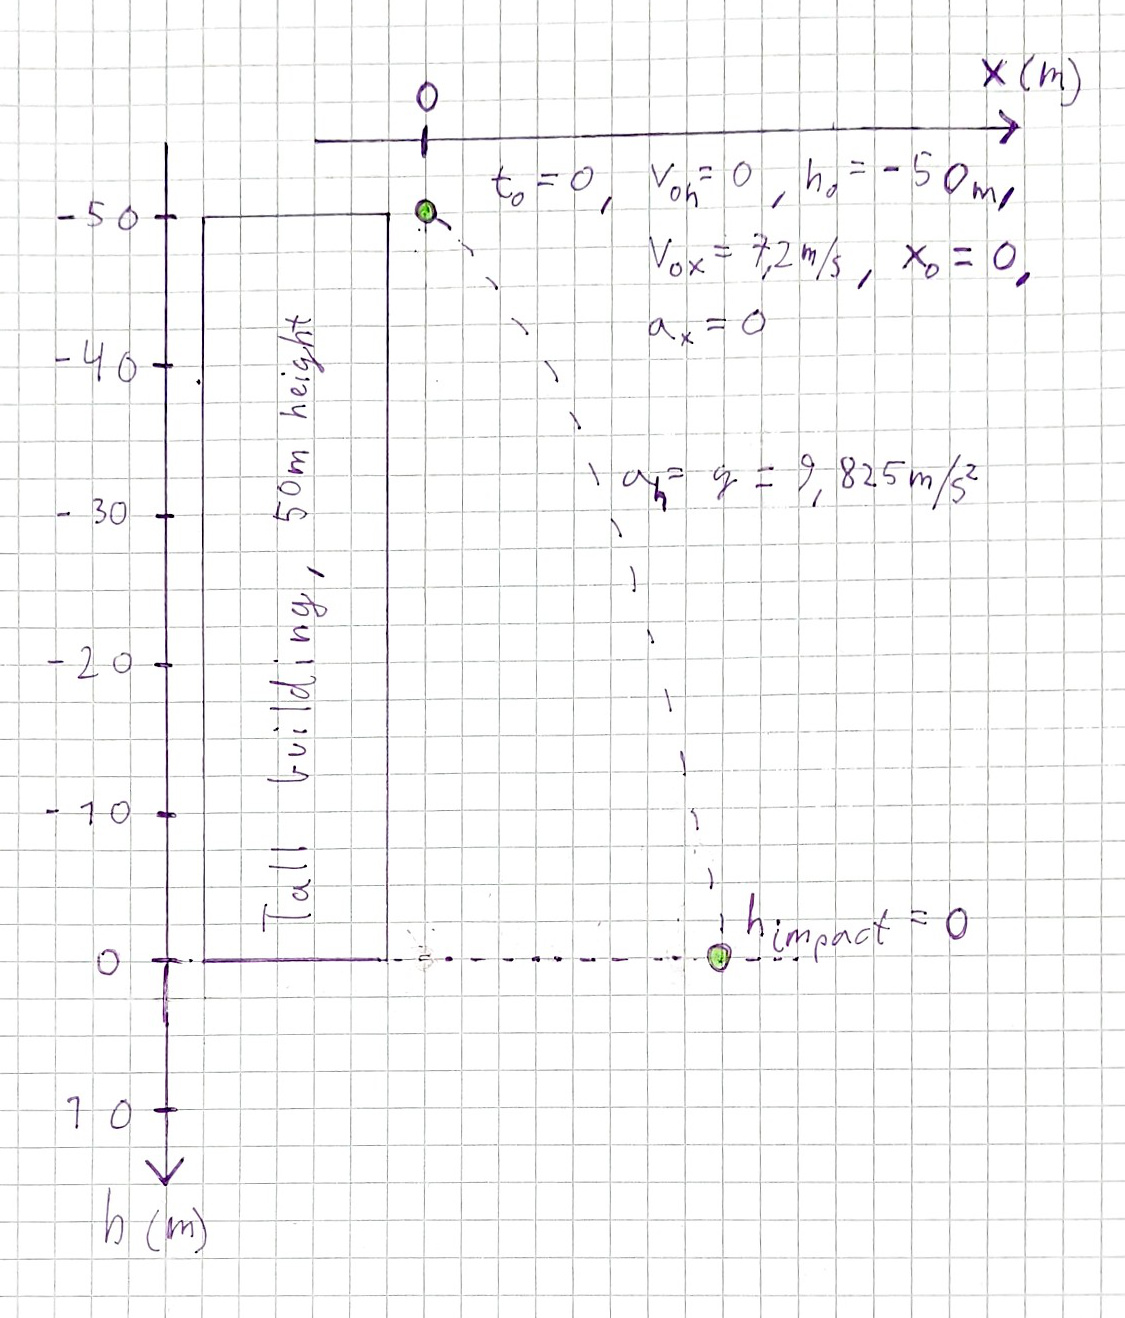
\includegraphics[width=0.6\textwidth]{Figures/Sketch2.jpg}
    \caption{Sketch of sphere falling with initial horizontal velocity}
    \label{fig:sketch_2}
\end{figure}

\subsubsection{Execute}
I start by simplifying this equation as both \(x_0 = 0\) and \(a_x = 0\) this removes two terms. Also filling in the used variables.

\begin{equation*}
    x_{impact} = v_0t_{impact}
\end{equation*}

Now with values is filled in.

\begin{equation}
    x_{impact} \approx 7.2ms^{-1} \cdot 3.19s \approx 22.97m
    \label{eq:x_impact}
\end{equation}

\clearpage
\subsubsection{Evaluate}
I feel like the magnitude of my answer is in the correct order and \(22.97m\) seems quite reasonable for an object to move that distance when the velocity is \(v_0 = 7.2ms^{-1}\), and travels for \(t_{impact} = 3.19s\). I will also want to check units to Equation~\ref{eq:x_impact}.

\begin{equation*}
    m = m \cdot s^{-1} \cdot s
\end{equation*}

\begin{equation*}
    m = m
\end{equation*}

Here the units check out. This makes me conclude that the answer is correct with a very high probability.

\subsubsection{Solution}
The sphere hits the ground after approximately \(3.19s\), the same as in part a.
\begin{equation*}
    t = \pm \sqrt{\frac{100m}{9.825ms^{-2}}} \approx 3.19s
    \tag{\ref{eq:t_impact}}
\end{equation*}
The sphere moved approximately \(22.97m\) horizontaly.
\begin{equation*}
    x_{impact} \approx 7.2ms^{-1} \cdot 3.19s \approx 22.97m
    \tag{\ref{eq:x_impact}}
\end{equation*}


\clearpage
\subsection{Part c}
To solve part c I choose to use the ISEE method.

\subsubsection{Identify}
This part does not need any numerical values as the task is to make a drawing, and set up an equation, therefore no important known values are needed. It is specified that correct sign should be used such that positive direction is upwards.

\subsubsection{Set up}
I start with the free body diagram, as it provides some context.

\begin{figure}[h]
    \centering
    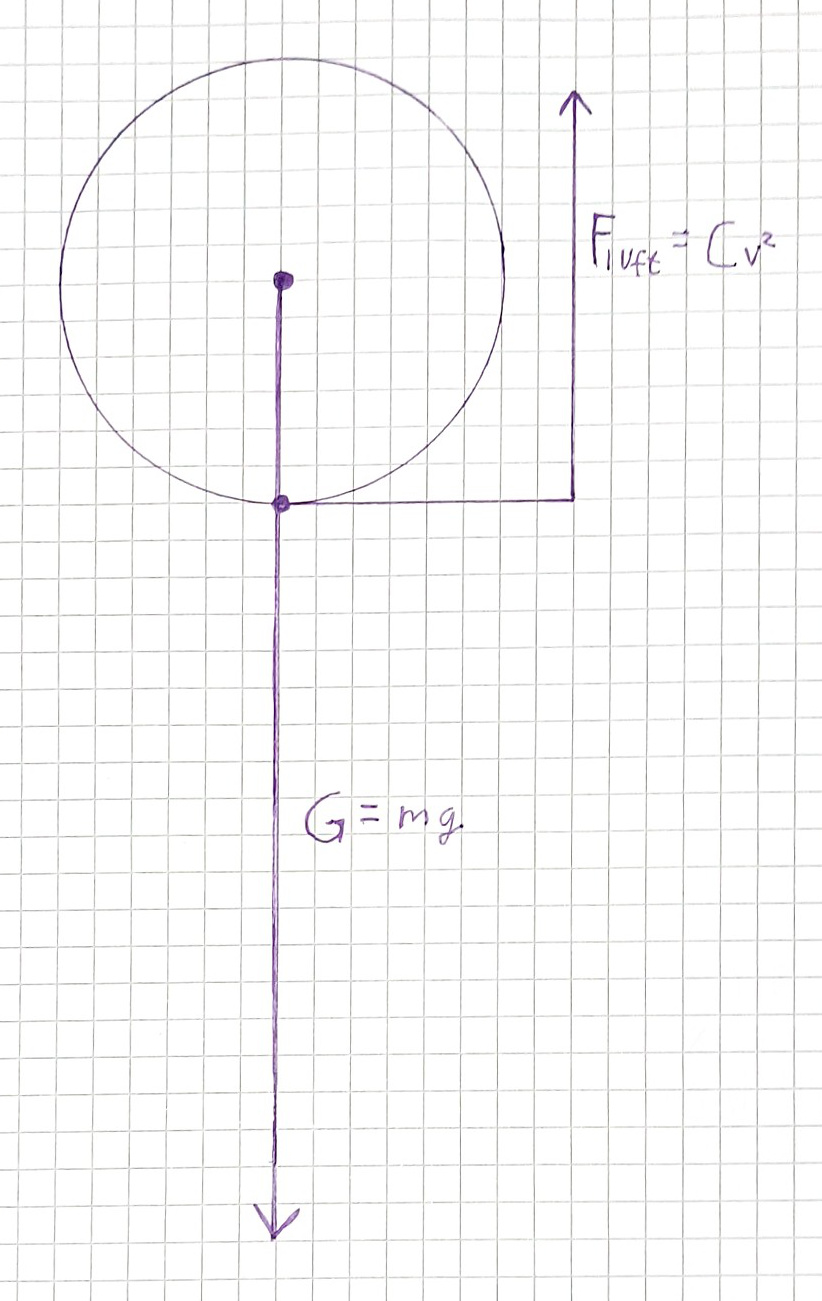
\includegraphics[width=0.6\textwidth]{Figures/Forces.jpg}
    \caption{Free body diagram of sphere with air resistance}
    \label{fig:Free_body_diagram}
\end{figure}
\clearpage
We only need to use one equation, Newtons 2nd law.

\begin{equation}
    \sum F = ma
    \label{eq:newton2}
\end{equation}

\subsubsection{Execute}

I start with modifying Equation~\ref{eq:newton2}, replacing the \(\sum F\) with the forces drawn in Figure~\ref{fig:Free_body_diagram}.

\begin{equation}
    F_{luft} - G = ma
    \label{eq:newton2_sphere}
\end{equation}

Now filling in for the forces and doing general arithmetic.

\begin{equation*}
    Cv^2 - mg = ma
\end{equation*}

\begin{equation*}
    \frac{Cv^2}{m} - g = a
\end{equation*}

\begin{equation}
    a = \frac{dv}{dt} = - g + \frac{Cv^2}{m}
    \label{eq:differnetial}
\end{equation}


\clearpage
\subsubsection{Evaluate}
In Figure~\ref{fig:Free_body_diagram} I made \(G\) larger than \(F_{luft}\) as without high starting speed or other forces, \(F_{luft}\) can never be larger than \(G\). Checking units for Equaton~\ref{eq:differnetial}.

\begin{equation*}
    m \cdot s^{-2} = m \cdot s^{-2} + \frac{kg \cdot m^{-1} \cdot (m \cdot s^{-1})^2}{kg}
\end{equation*}

\begin{equation*}
    m \cdot s^{-2} = m \cdot s^{-2} + m^{-1} \cdot m^2 \cdot s^{-2}
\end{equation*}

\begin{equation*}
    m \cdot s^{-2} = m \cdot s^{-2} + m \cdot s^{-2}
\end{equation*}


\begin{equation*}
    m \cdot s^{-2} = m \cdot s^{-2} 
\end{equation*}

Here the units checks out. This makes me conclude that the answer is correct with a very high probability.

\subsubsection{Solution}
Free body diagram is drawn in Figure~\ref{fig:Free_body_diagram}.\\
\\
Newtons 2nd law for this situation:
\begin{equation*}
    F_{luft} - G = ma
    \tag{\ref{eq:newton2_sphere}}
\end{equation*}

Can be rewritten to this:
\begin{equation*}
    a = \frac{dv}{dt} = - g + \frac{Cv^2}{m}
    \tag{\ref{eq:differnetial}}
\end{equation*}


\clearpage
\subsection{Part d}
To solve part d I choose to use the ISEE method and use results from part c.

\subsubsection{Identify}
I find \(v_T\) to be the terminal velocity. I also find a value for \(C = 5.00 \cdot 10^{-2} kgm^{-1}\) and \(m = 100g\). I need to use Equation~\ref{eq:differnetial} from part c.

\subsubsection{Set up}
The first thing to do is to correct \(m = 100g\) into \(m = 0.1kg\) such as to keep all units as SI-units. Terminal velocity will cause no acceleration as there is no change in speed, this means that \(\frac{dv}{dt}=0\) at terminal velocity. It can be set up like this.

\begin{equation*}
    0 = - g + \frac{Cv^2}{m}
\end{equation*}

\subsubsection{Execute}
solving this for \(v\) using arithmetic.

\begin{equation*}
    g = \frac{Cv^2}{m}
\end{equation*}

\begin{equation*}
    mg = Cv^2
\end{equation*}

\begin{equation*}
    \frac{mg}{C} = v^2
\end{equation*}

\begin{equation}
    v = \pm\sqrt{\frac{mg}{C}}
    \label{eq:v_terminal}
\end{equation}

Only the negative answer makes sense with positive direction upwards. Filling in values for \(m\), \(g\) and \(C\).

\begin{equation}
    v = -\sqrt{\frac{0.1kg \cdot 9.825 ms^{-2}}{5.00 \cdot10^{-2}kgm^{-1}}} \approx -4.43ms^{-1}
    \label{eq:v_terminal_sphere}
\end{equation}

\clearpage
\subsubsection{Evaluate}
I feel like the magnitude of my answer is in the correct order and \(-4.43ms^{-1}\) seems quite reasonable terminal speed for a object with mass \(m = 100g\), it is maybe a bit slower than intuitivly expected for me. I will also want to check units for Equation~\ref{v_terminal_sphere}.

\begin{equation*}
    m \cdot s^{-1} = \sqrt{\frac{kg \cdot m \cdot s^{-2}}{kg \cdot m^{-1}}}
\end{equation*}

\begin{equation*}
    m \cdot s^{-1} = \sqrt{\frac{m \cdot s^{-2}}{m^{-1}}}
\end{equation*}

\begin{equation*}
    m \cdot s^{-1} = \sqrt{m^2 \cdot s^{-2}}
\end{equation*}

\begin{equation*}
    m \cdot s^{-1} = \sqrt{\frac{m^2}{s^2}}
\end{equation*}

\begin{equation*}
    m \cdot s^{-1} = \frac{m}{s}
\end{equation*}

\begin{equation*}
    m \cdot s^{-1} = m \cdot s^{-1}
\end{equation*}

\subsubsection{Solution}
Using Equation~\ref{eq:differnetial} with \(\frac{dv}{dt}=0\) you can get equation for terminal velovity.

\begin{equation*}
    v = \pm\sqrt{\frac{mg}{C}}
    \tag{\ref{eq:v_terminal}}
\end{equation*}

Filling in values for c we find that the teminal velocity is approximately \(-4.43ms^{-1}\).

\begin{equation*}
    v = -\sqrt{\frac{0.1kg \cdot 9.825 ms^{-2}}{5.00 \cdot10^{-2}kgm^{-1}}} \approx -4.43ms^{-1}
    \tag{\ref{eq:v_terminal_sphere}}
\end{equation*}

\section{Task 2}
Now I may have overdone this section as I taught this was a good exercise to extend my python skills, in other words, the code does exactly as described, and more. But it does not reassemble the example code a whole lot. If clarifications on how the code works is needed, feel free to reach out.
In general the code as shown in Subsection~\ref{subsection:code} runs two simulations one with positive direction upwards named Sphere 1 and one with positive direction downwards, named Sphere 2 as the program handles both.

\clearpage
\subsection{Part a}
\begin{figure}[h]
    \centering
    \begin{subfigure}{0.8\textwidth}
        \centering
        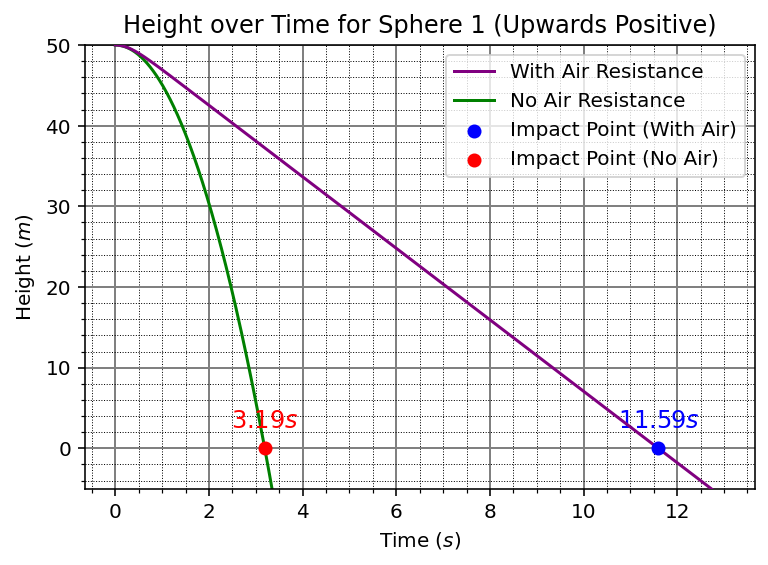
\includegraphics[width=1\textwidth]{Figures/ht1.png}
    \end{subfigure}
    \begin{subfigure}{0.8\textwidth}
        \centering
        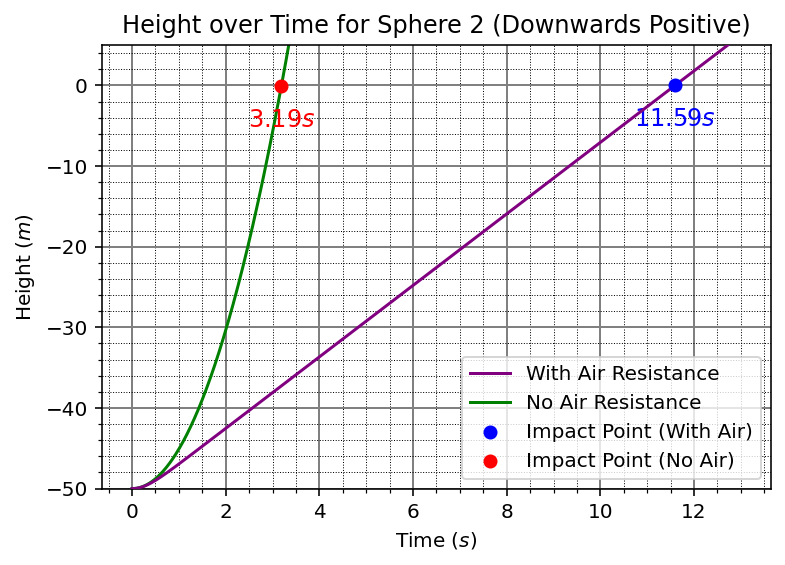
\includegraphics[width=1\textwidth]{Figures/ht2.png}
    \end{subfigure}
    \caption{Simulations of height both with and without air resistance}
    \label{fig:sim_h}
\end{figure}

\clearpage
\subsection{Part b}
\begin{figure}[h]
    \centering
    \begin{subfigure}{0.8\textwidth}
        \centering
        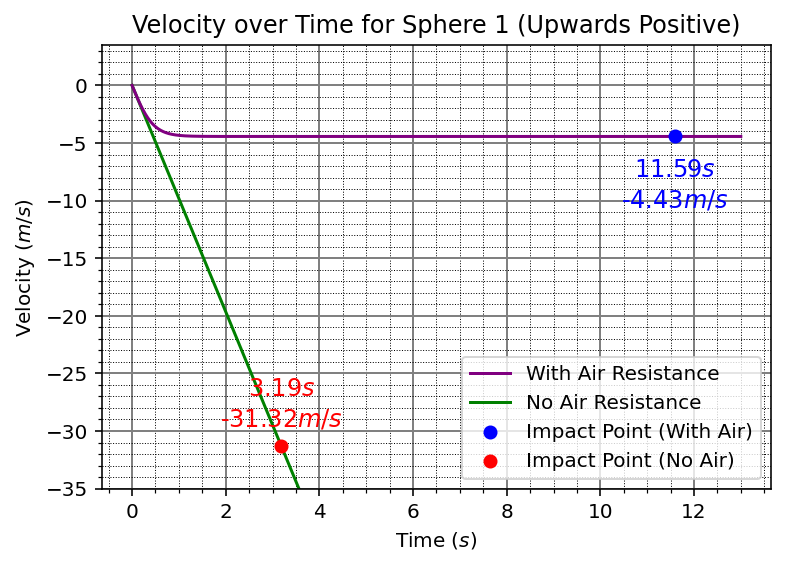
\includegraphics[width=1\textwidth]{Figures/vt1.png}
    \end{subfigure}
    \begin{subfigure}{0.8\textwidth}
        \centering
        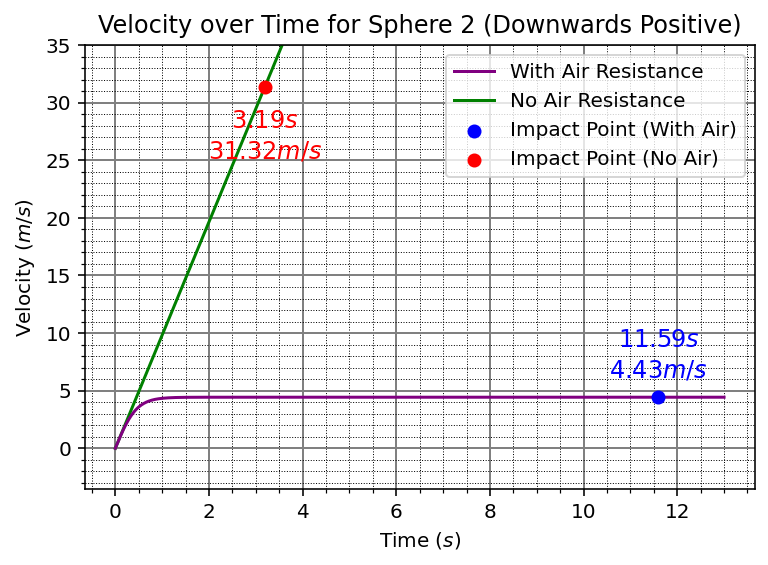
\includegraphics[width=1\textwidth]{Figures/vt2.png}
    \end{subfigure}
    \caption{Simulations of velocity both with and without air resistance}
    \label{fig:sim_v}
\end{figure}

\subsection{Part c}
We can see from the graph that terminal velocity \(v_T\) is achieved and the size is \(4.43ms^{-1}\). This corresponds well with results of Equation~\ref{eq:v_terminal_sphere}

\begin{equation*}
    v = -\sqrt{\frac{0.1kg \cdot 9.825 ms^{-2}}{5.00 \cdot10^{-2}kgm^{-1}}} \approx -4.43ms^{-1}
    \tag{\ref{eq:v_terminal_sphere}}
\end{equation*}

\clearpage
\subsection{Ekstra}
\begin{figure}[h]
    \centering
    \begin{subfigure}{0.8\textwidth}
        \centering
        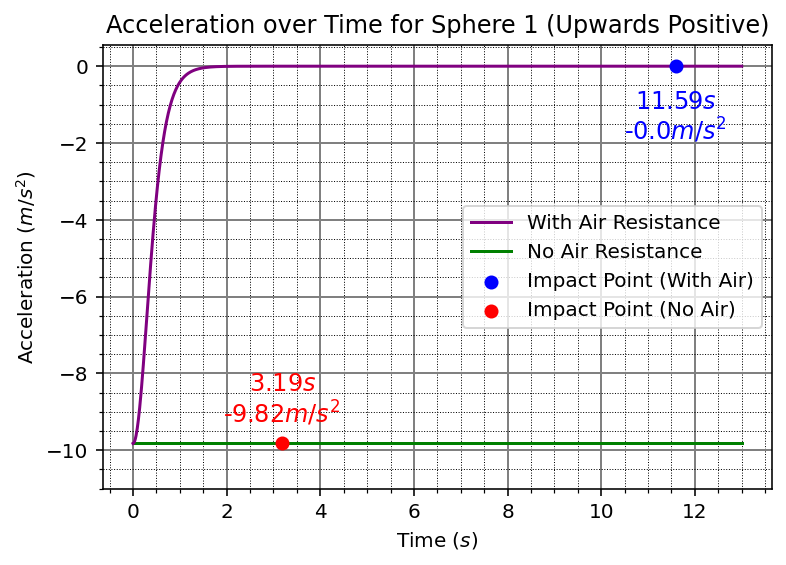
\includegraphics[width=1\textwidth]{Figures/at1.png}
    \end{subfigure}
    \begin{subfigure}{0.8\textwidth}
        \centering
        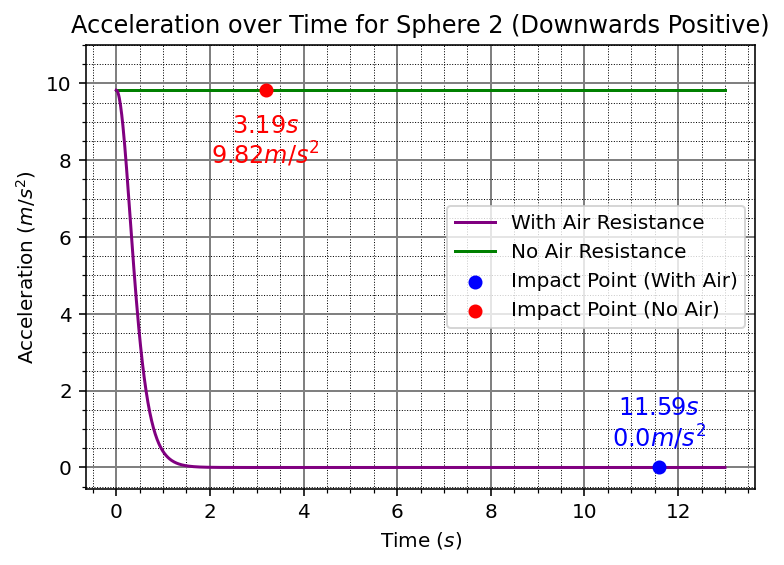
\includegraphics[width=1\textwidth]{Figures/at2.png}
    \end{subfigure}
    \caption{Simulations of acceleration both with and without air resistance}
    \label{fig:sim_a}
\end{figure}

\clearpage
\subsection{Source code} \label{subsection:code}
\writecode[Python]{Simulator.py}{Simulation of falling spheres, over engineered to a high degree}

\end{document}
